\documentclass[a4paper,12pt]{article} %style de document
\usepackage[utf8]{inputenc} %encodage des caractères
\usepackage[french]{babel} %paquet de langue français
\usepackage[T1]{fontenc} %encodage de la police
\usepackage[top=2cm,bottom=2cm,left=2cm,right=2cm]{geometry} %marges
\usepackage{graphicx} %affichage des images
\usepackage{wrapfig} %Images à côté du texte
\usepackage{url}

\begin{document} %début du document

%page de garde
\begin{titlepage}
\begin{center}
\Large{Année universitaire 2016-2017}\\
\Large{Université de Caen Basse-Normandie}\\[1cm]
\Large{20 Septembre 2016}\\
\Large{Groupe 3}\\
\vspace{5cm}
\huge{RAPPORT N\up{o}1 DU PROJET DE TPA :}\\
L'IDE\\
\normalsize{\textit{ ~ Itegrated Developpement Environement}}\\
\vspace{5cm}
\huge{}
Alexis Carreau\\
Thomas Lécluse\\
Emma Mauger\\
Théo Sarrazin\\
\normalsize{\textit{ ~ L2 Informatique}}\\
\medskip
\vspace{2cm}

\end{center}
\end{titlepage}

\newpage

Dans ce premier rapport nous présentons l’architecture contenant le cahier des charges ainsi que l’arborescence de l’IDE. Il sera également possible de sauvegarder le travail effectué. L’éditeur de texte devra gérer l’auto-complétion et mettre en évidence les mots-clés et les variables ainsi qu’une liste des classes, leurs attributs et leurs méthodes. Durant cette première phase nous allons réaliser un IDE qui coloriera automatiquement les mots-clés et nous effectuons une recherche bibliographique et technologique, il s’agit de la réalisation d’un prototype. Actuellement, nous avons géré le traitement des couleurs sur notre IDE, c’est-à-dire la reconnaissance des balises et leur coloration. Nous avons également mis en place un système de chargement et sauvegarde de fichiers ainsi que la mise à jour du navigateur. Enfin, au niveau de l'interface graphique, nous retrouvons un navigateur de fichier, un aperçu du rendu et l’éditeur de texte contenant le code, ainsi qu'un menu de navigation. Nous avons choisi ce sujet puisqu’il est intéressant de travailler avec nos propres outils afin de concevoir des programmes.

\vspace{3cm}

\begin{figure}[h!]
	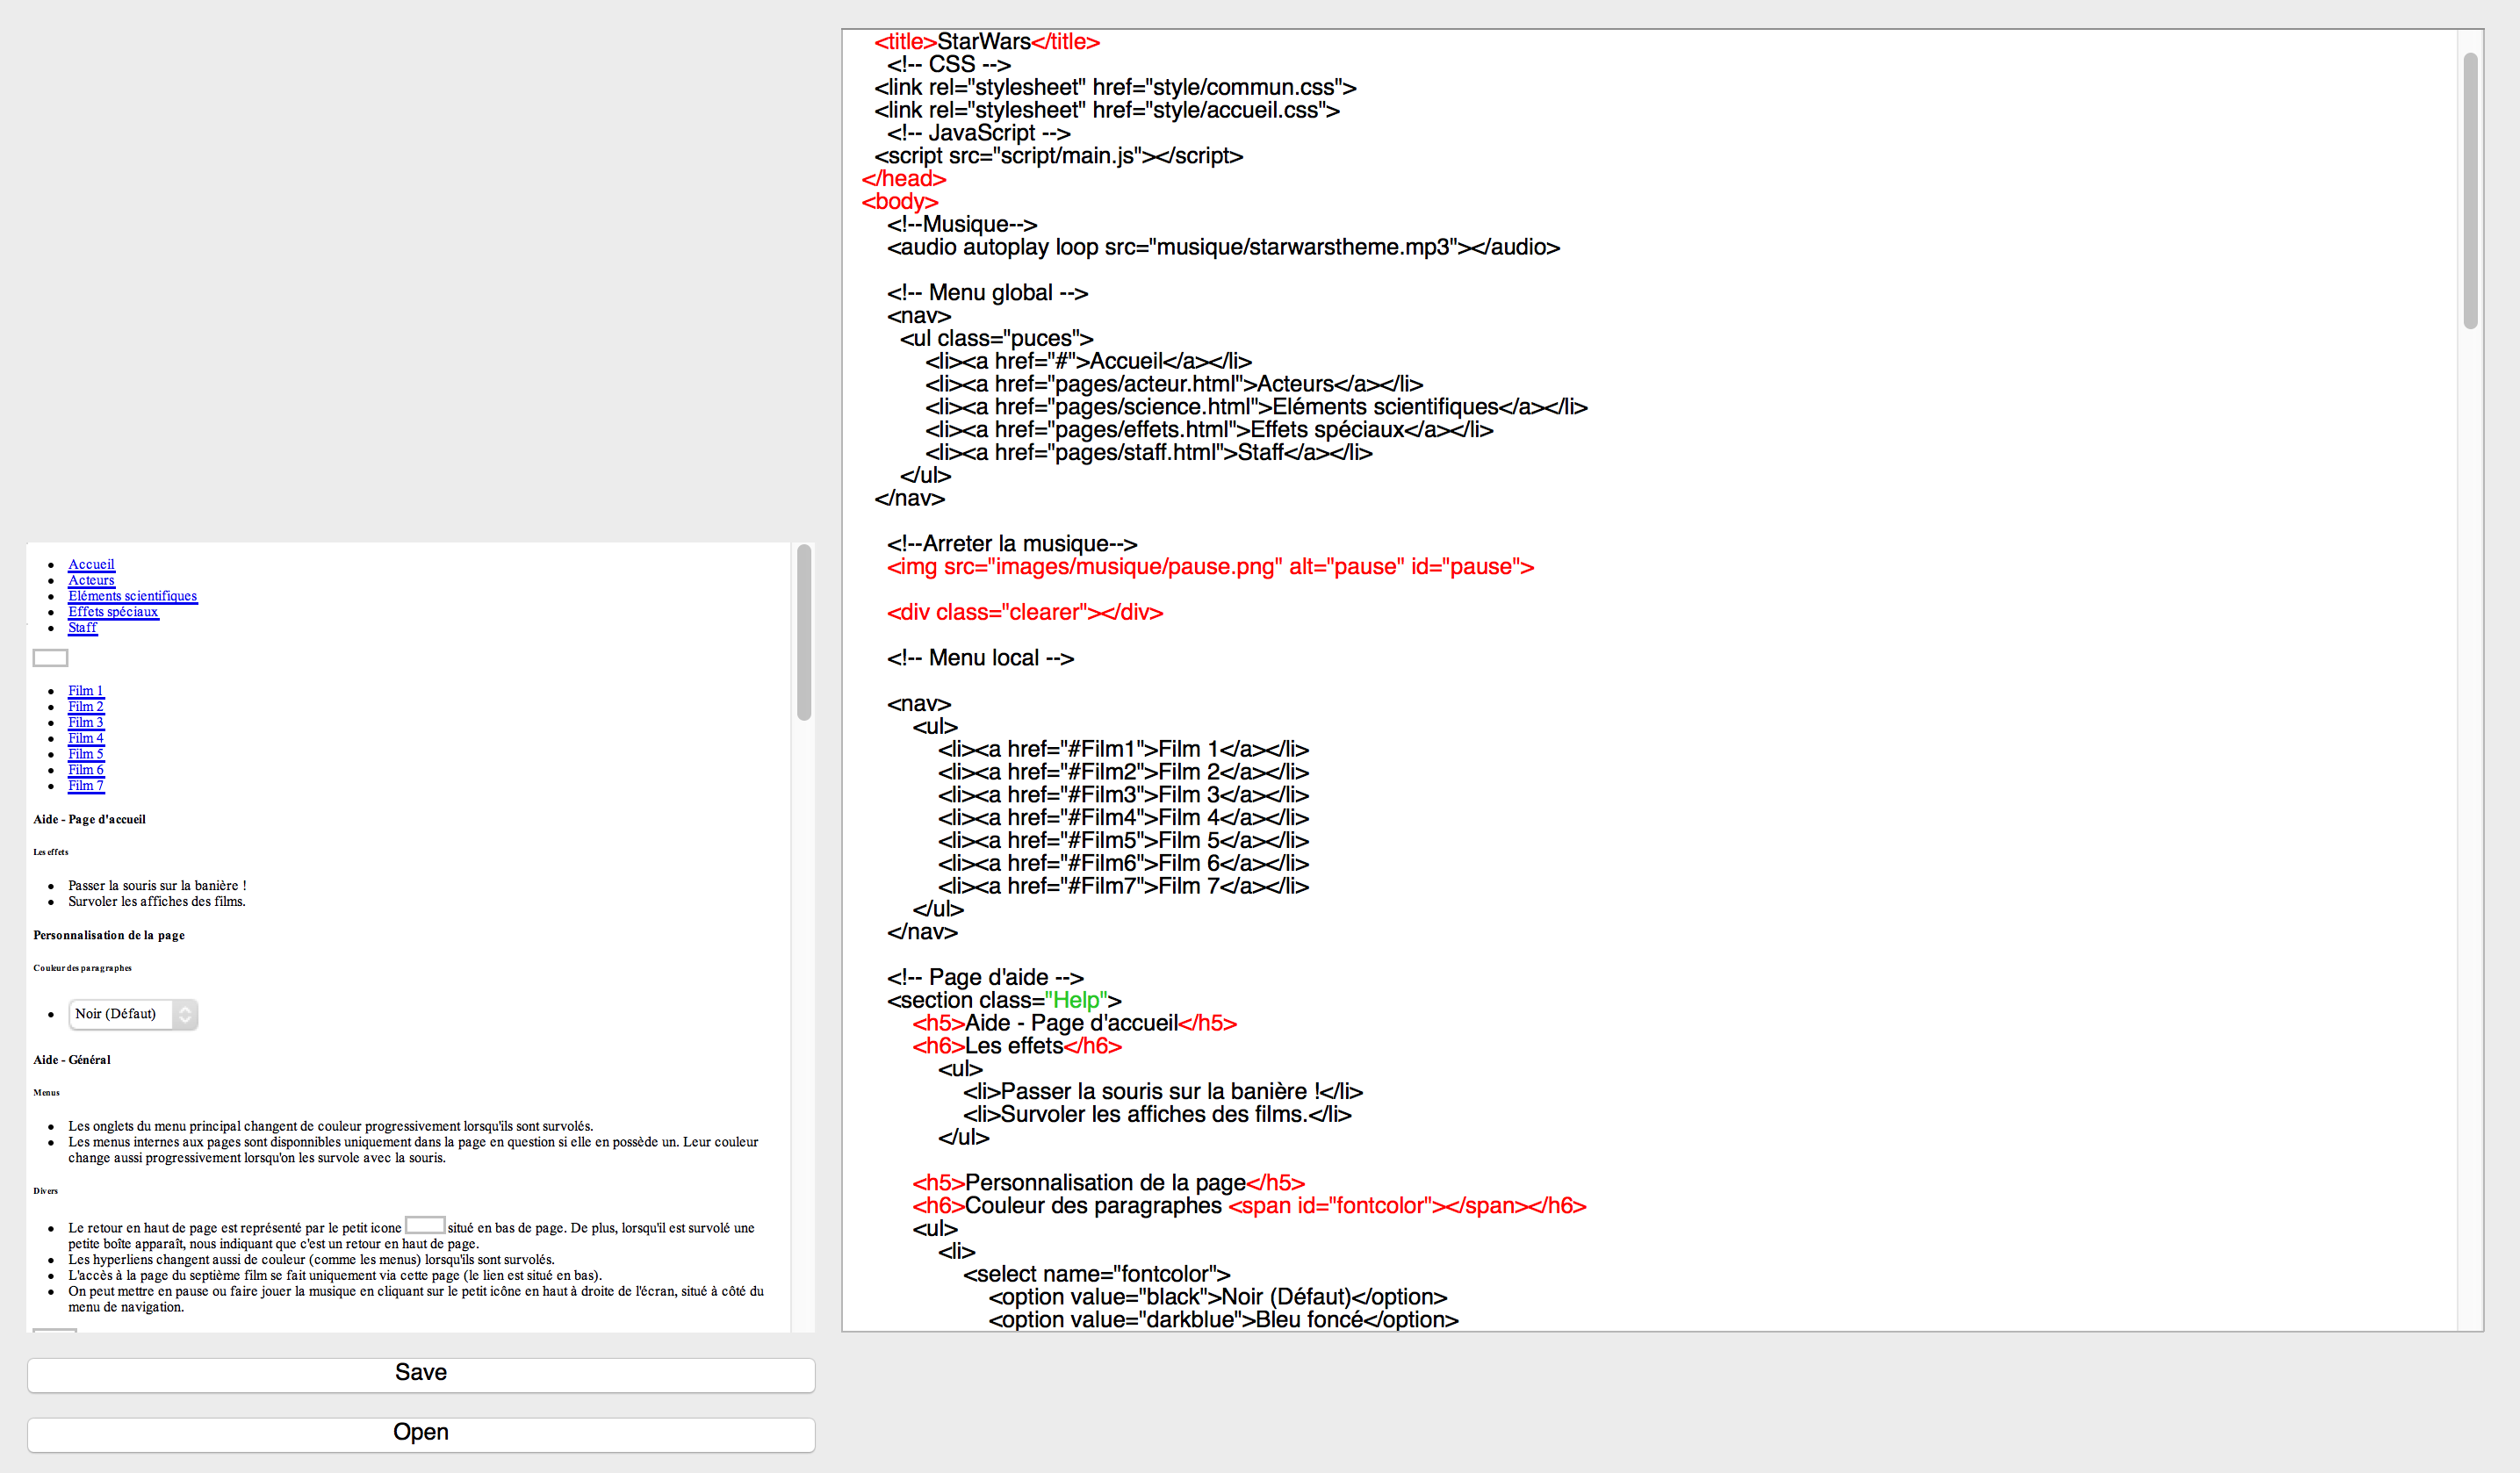
\includegraphics[scale=0.35]{images/IDE.png}
	\caption{Aperçu de l'IDE}
\end{figure}



\end{document}